\documentclass[landscape]{article}
\usepackage[pdftex]{graphicx}
\pagestyle{empty}
\oddsidemargin  -0.5 in
\evensidemargin -0.5 in
\headheight     0 in
\topmargin      -1 in
\textheight     7.7 in
\textwidth      10 in
\begin{document}
\huge
\renewcommand{\labelitemi}{-}
\setlength{\parindent}{0 cm}

\begin{center} 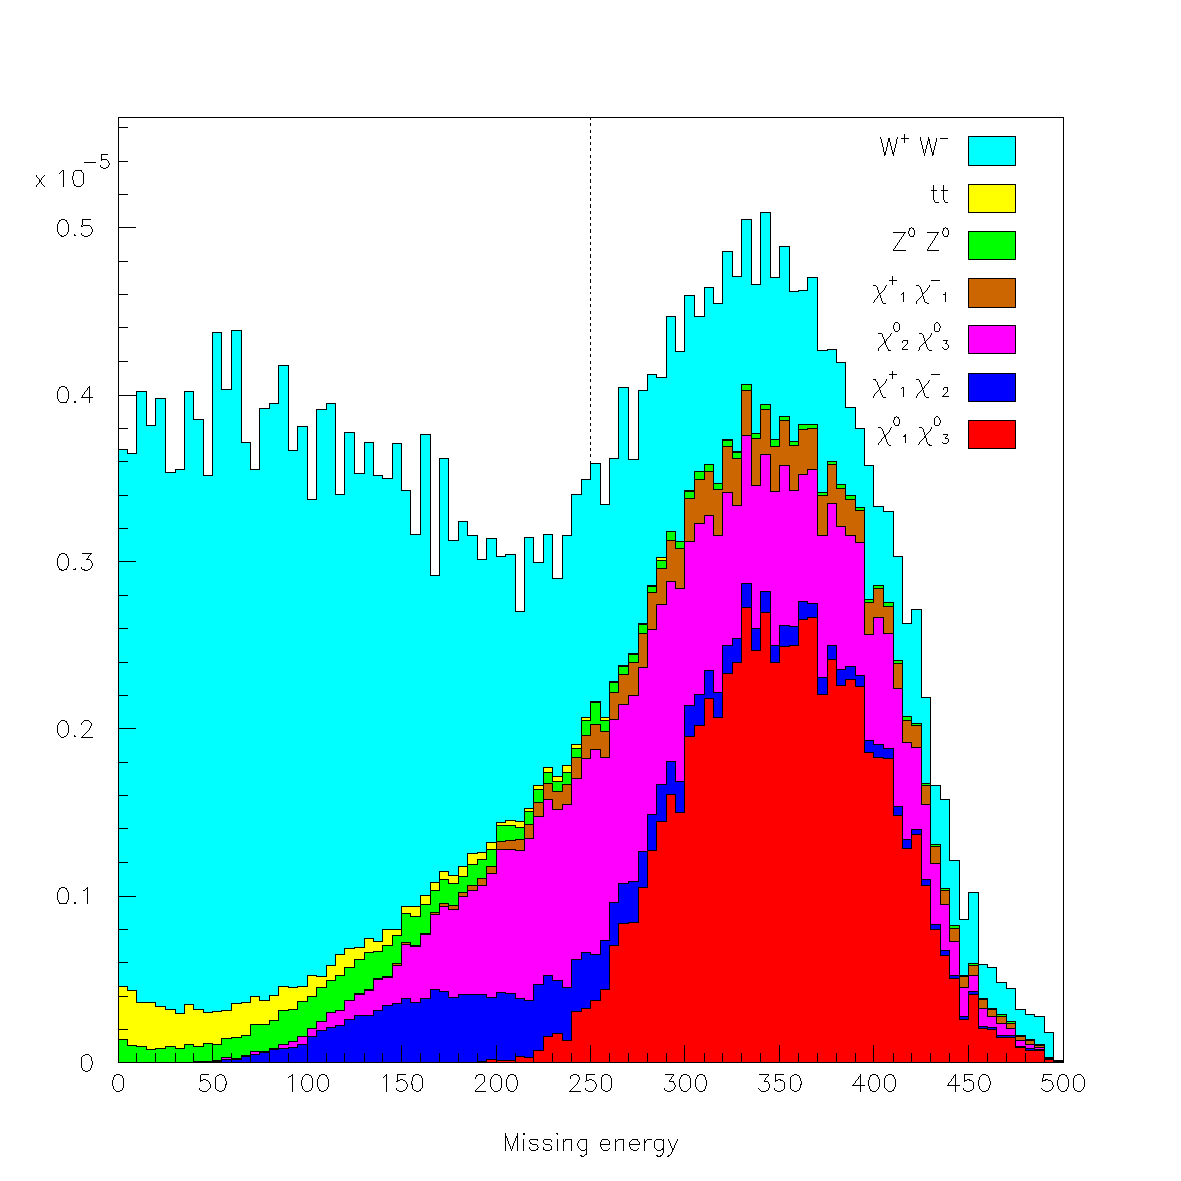
\includegraphics[height=0.8\textheight]{withtheta_1.pdf} \end{center}

The famous missing-energy plot.  Let's be more generous and only cut off $<$ 250 GeV.

\pagebreak

\begin{center} 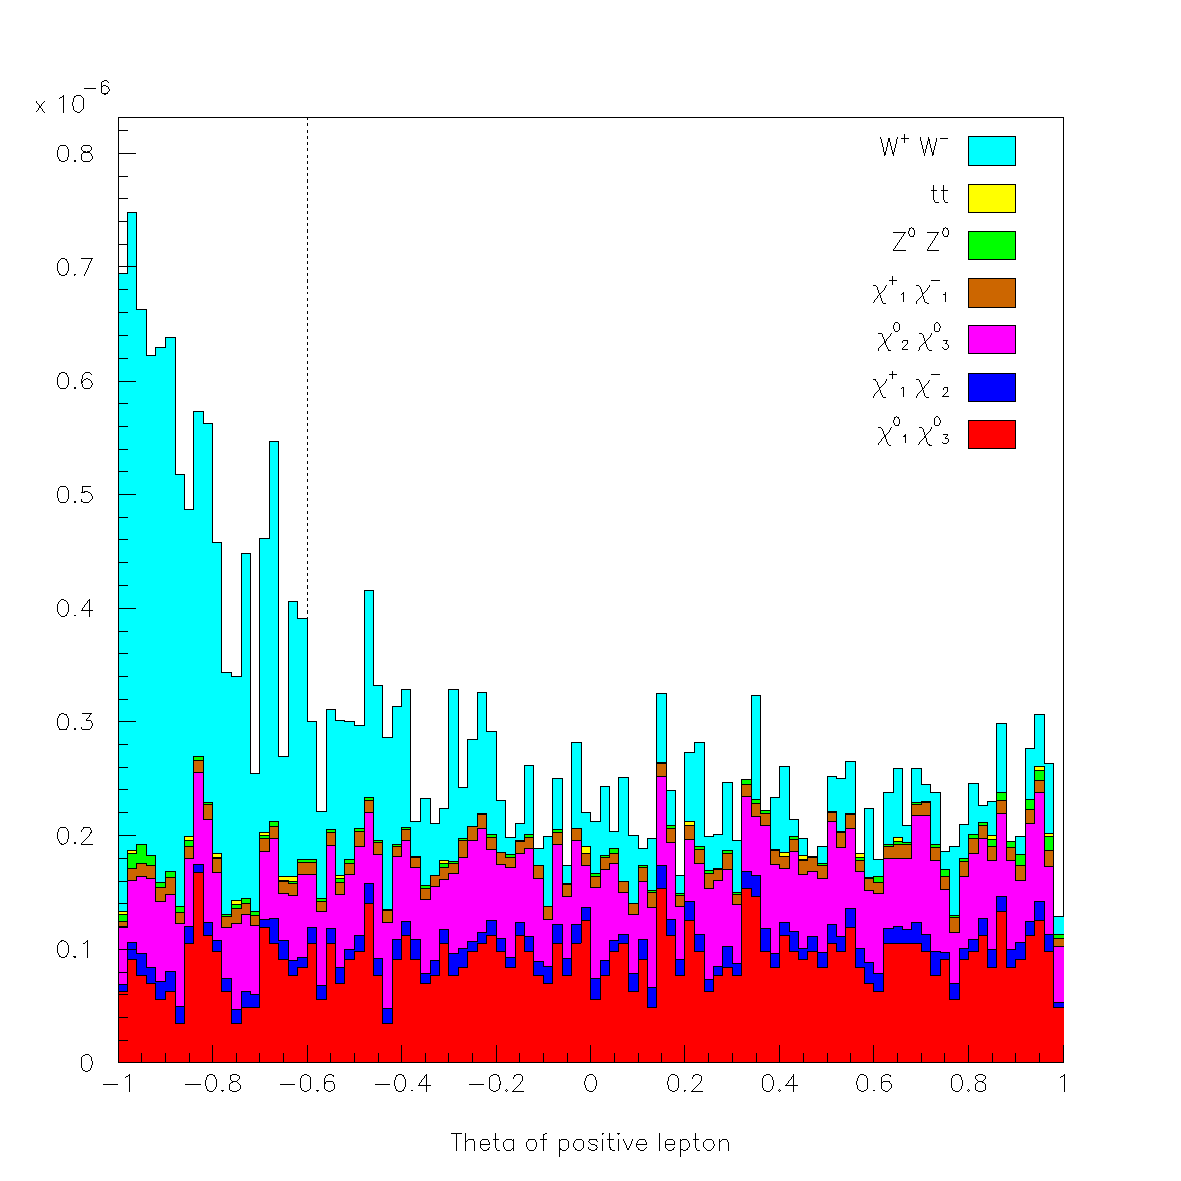
\includegraphics[height=0.8\textheight]{withtheta_2.pdf} \end{center}

This is cos($\theta$) of the positive lepton.  $W^+W^-$ events are
highly peaked at -1, and SUSY is flat, so I cut at -0.6.

\pagebreak

\begin{center} 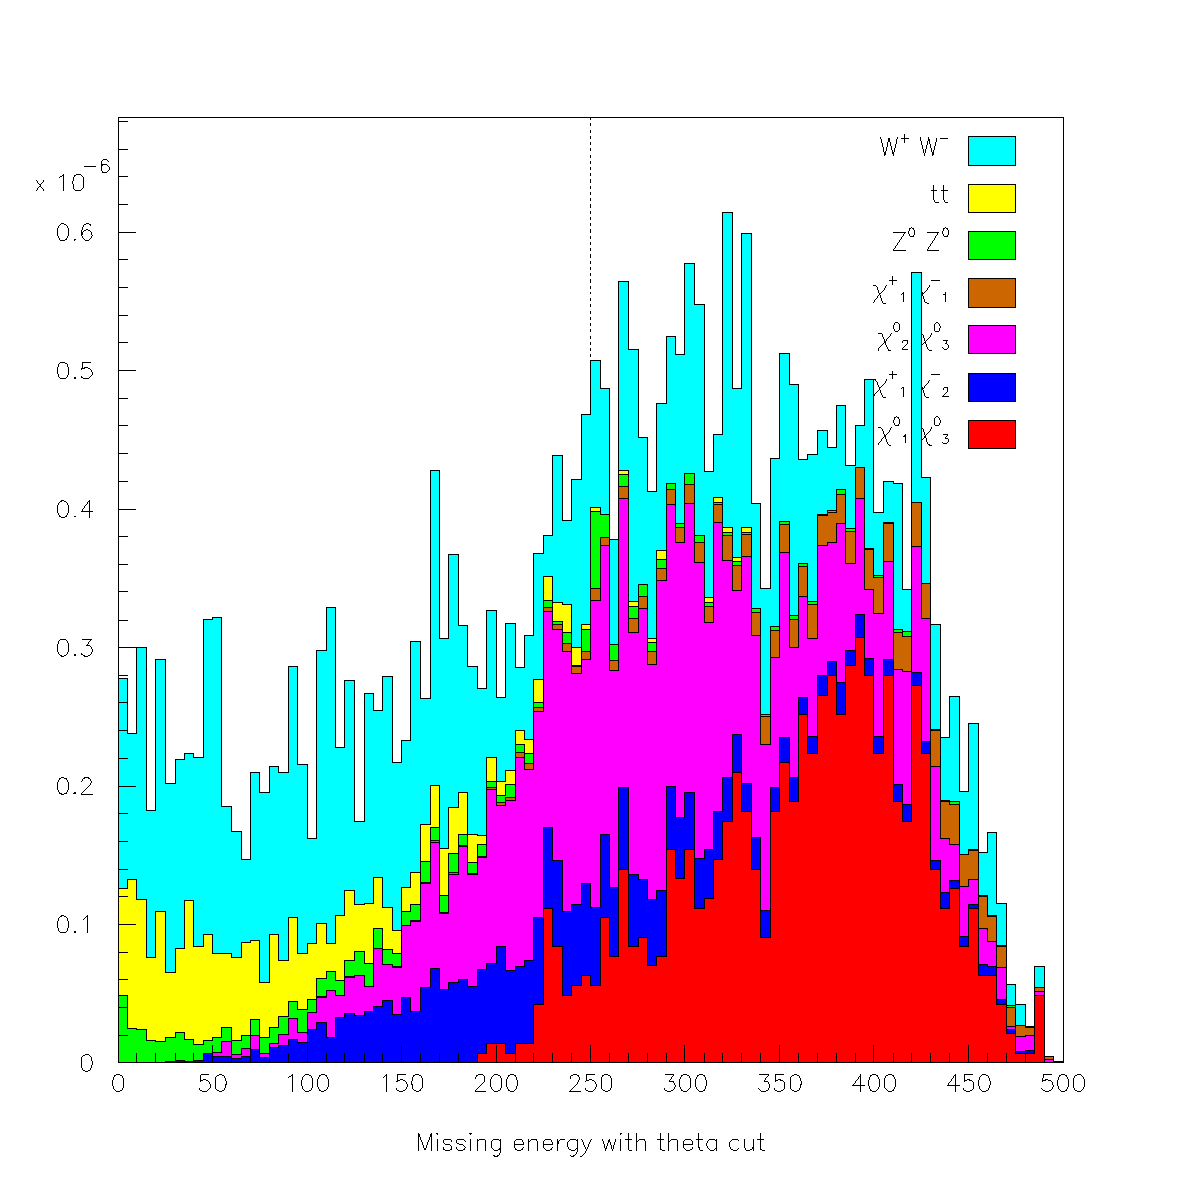
\includegraphics[height=0.8\textheight]{withtheta_3.pdf} \end{center}

Look at missing energy again, this time with the $\theta$ cut.

\pagebreak

\begin{center} 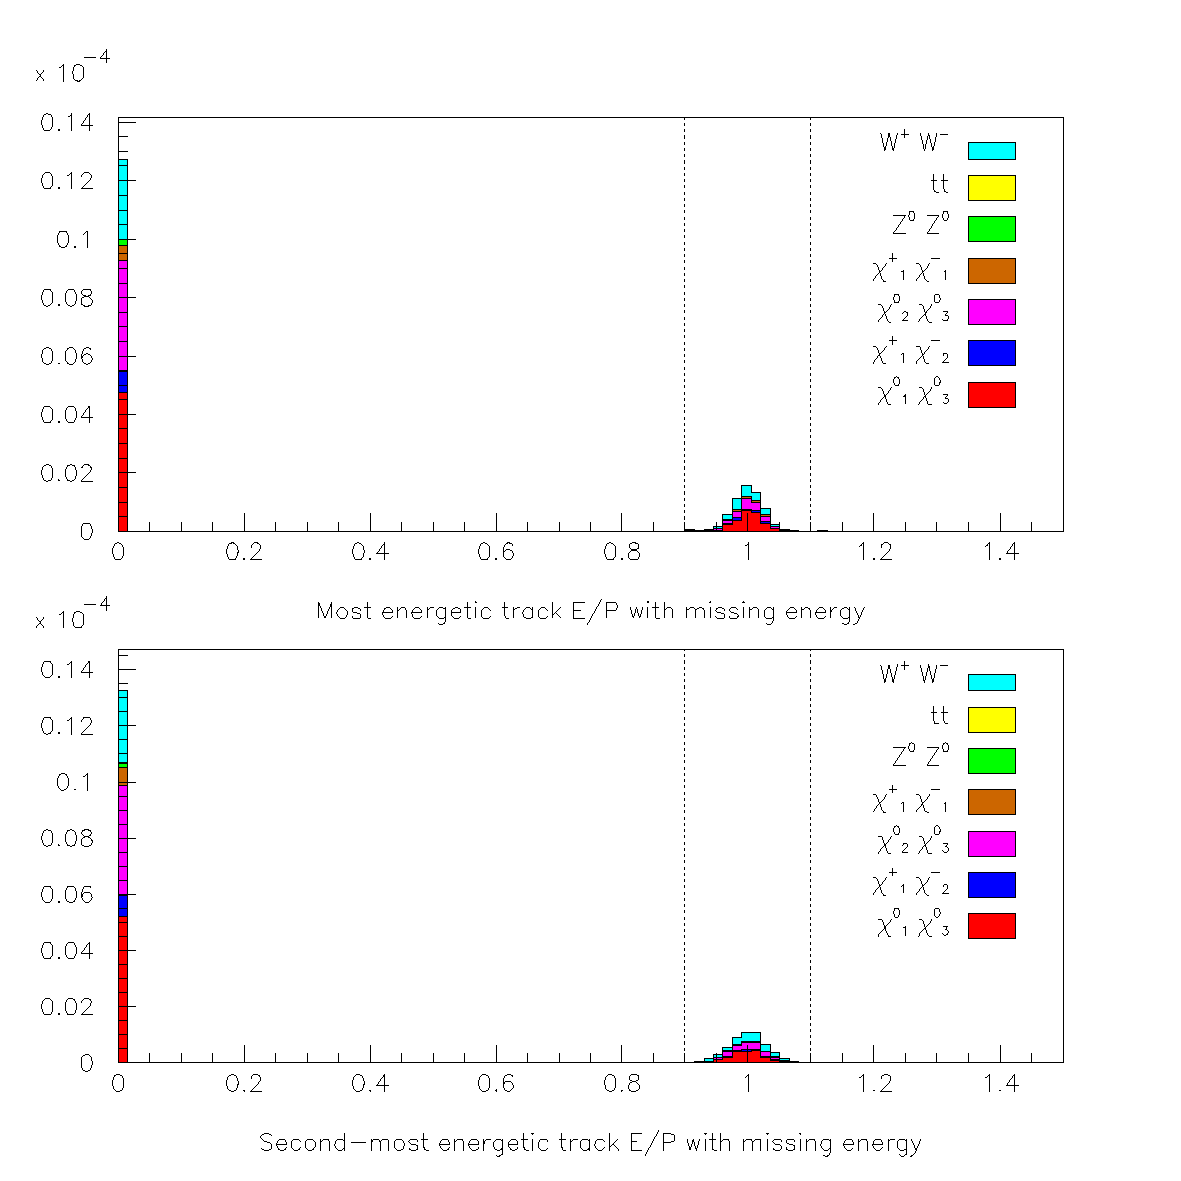
\includegraphics[height=0.8\textheight]{withtheta_4.pdf} \end{center}

Use track-cluster matching to pick out only $e^+e^-$.  This improves
$\mbox{$\chi^0$}_1 \mbox{$\chi^0$}_3 / W^+W^-$ signal-to-background by
a factor of two.  In the future, we will be able to cleanly identify
mupairs as well, so in the last few plots I'll multiply my results by
a factor of two.

\pagebreak

\begin{center} 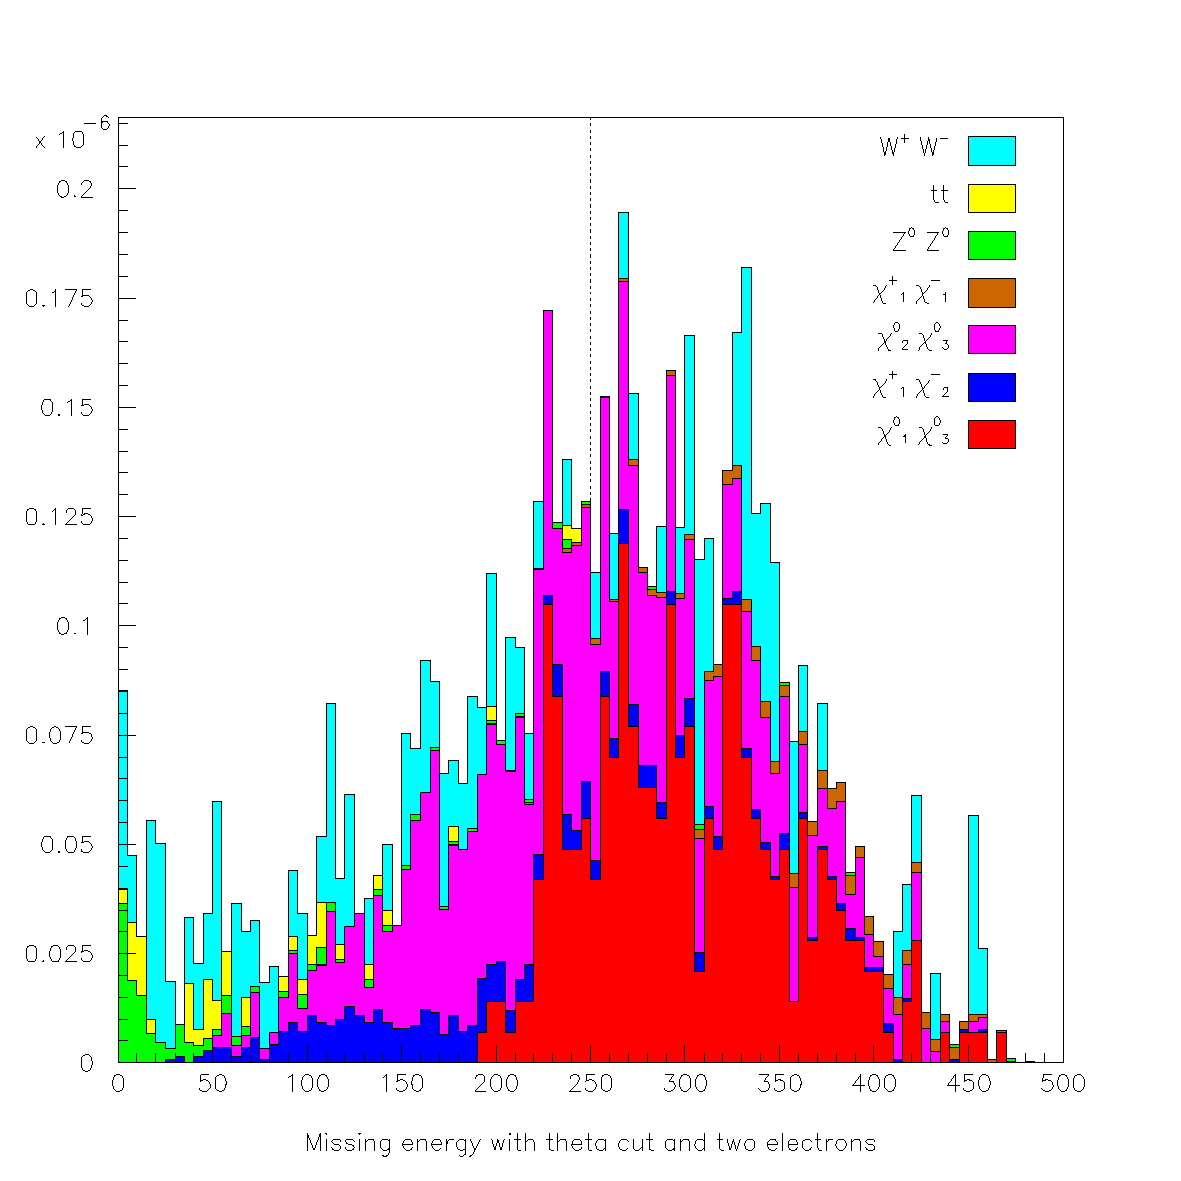
\includegraphics[height=0.8\textheight]{withtheta_5.pdf} \end{center}

Missing energy again, with all the accumulated cuts.

\pagebreak

\begin{center} 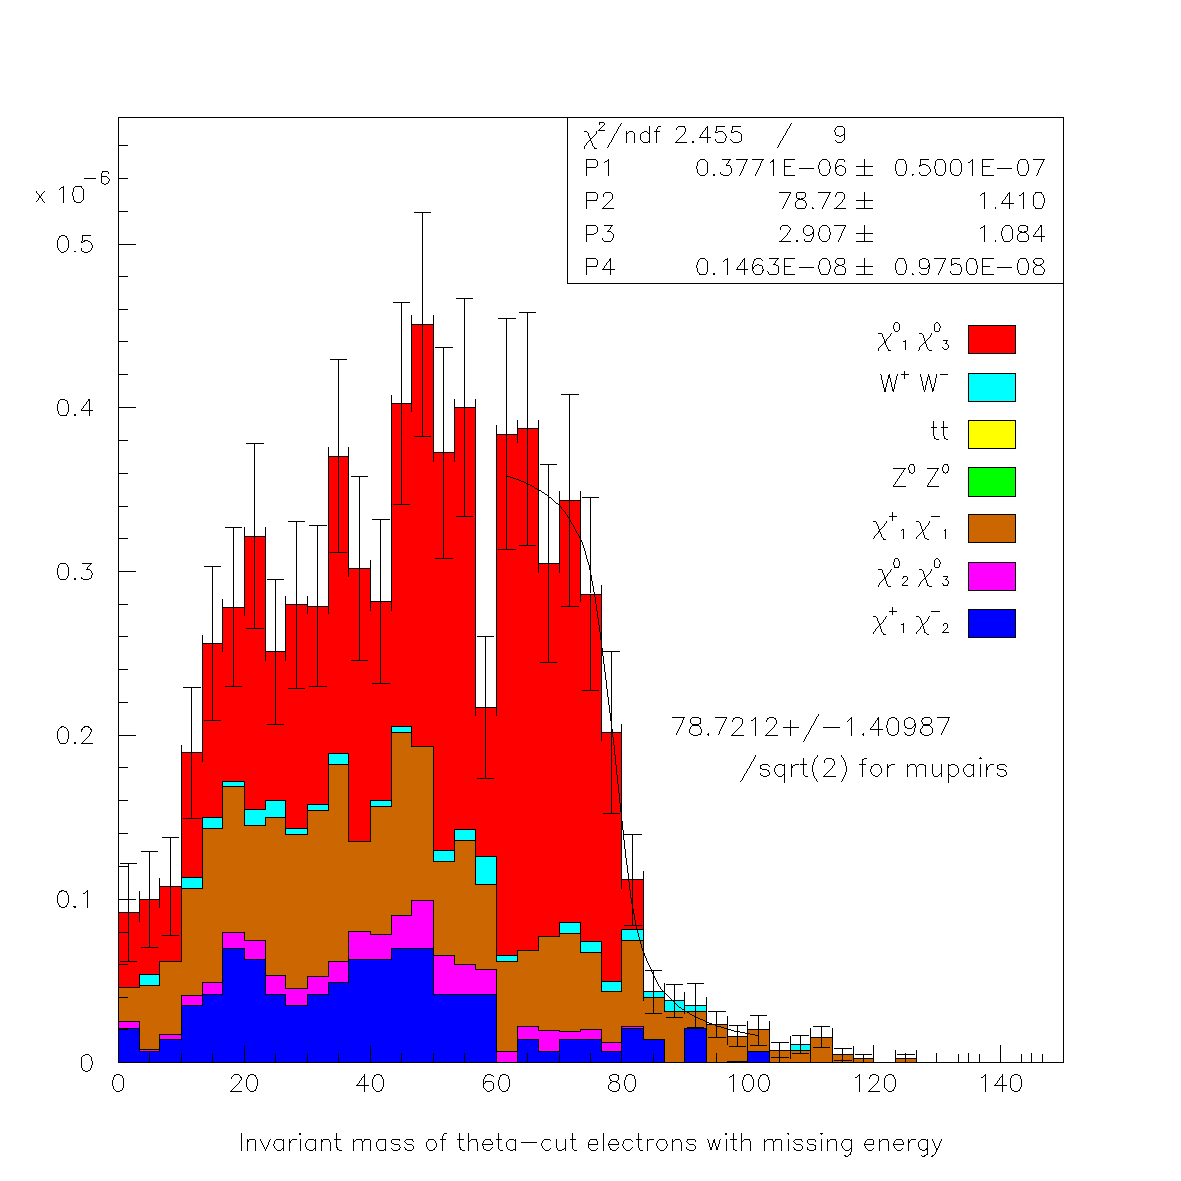
\includegraphics[height=0.8\textheight]{withtheta_6.pdf} \end{center}

This is the two-lepton mass distribution with all cuts, signal on top.
The backgrounds are now all SUSY, but they are rather flat in the
cut-off region.  Look: $\pm$ 1 GeV uncertainty!  But you have to model
backgrounds that you don't necessarily understand\ldots

\pagebreak

\begin{center} 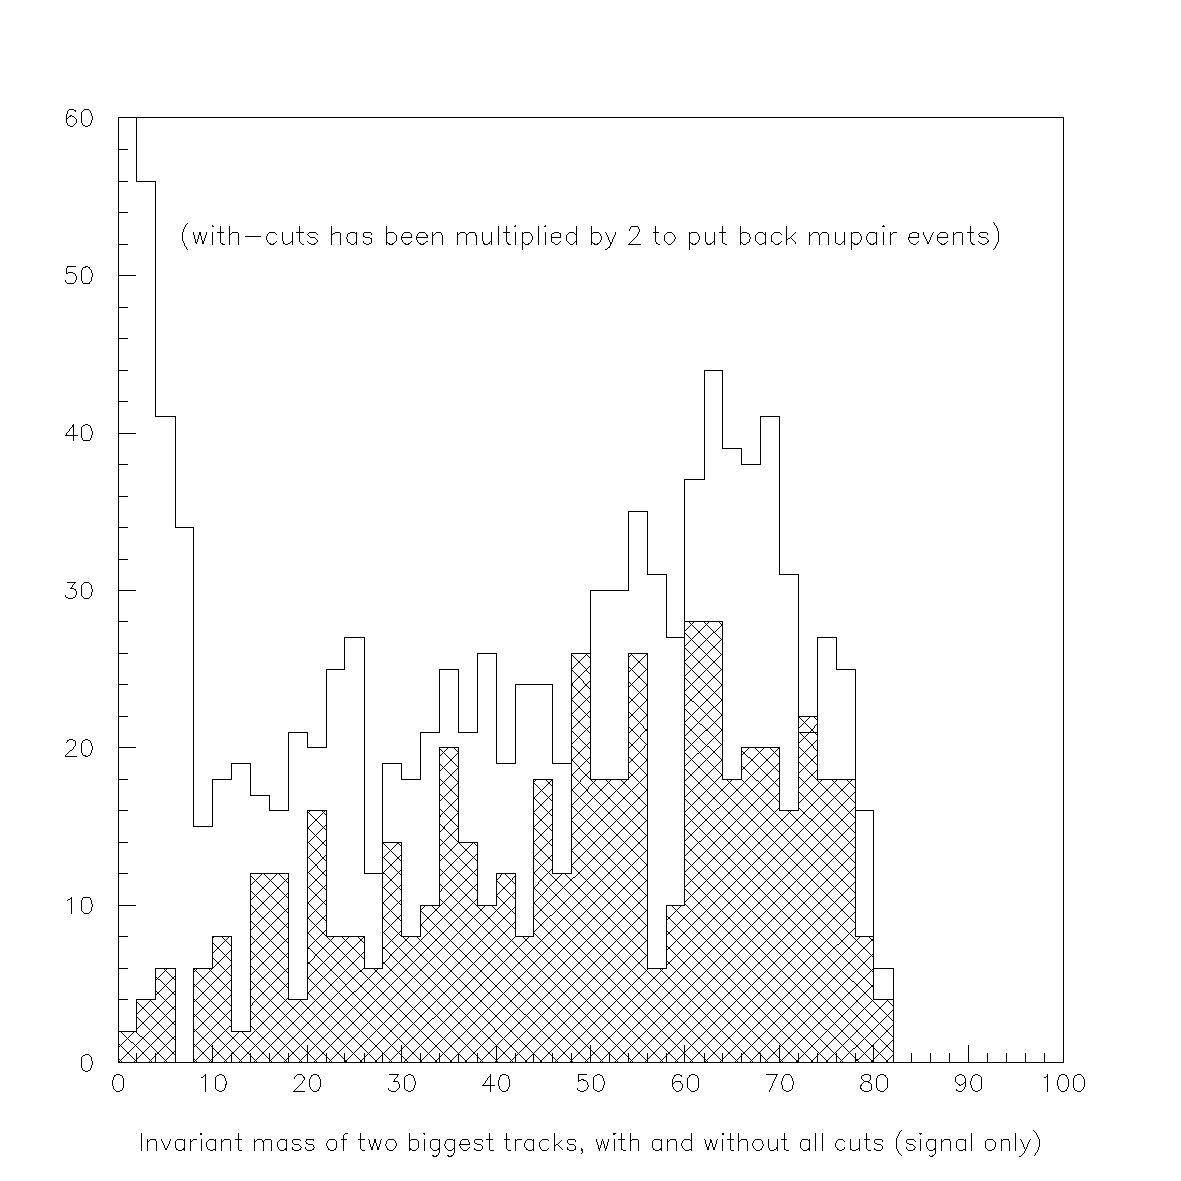
\includegraphics[height=0.8\textheight]{withtheta_7.pdf} \end{center}

The new cuts are much more efficient, if we assume we can put the
mupairs back in.  They also don't affect the location of the
two-lepton mass cut-off.


\end{document}
